\documentclass[11pt]{article}

\usepackage[margin=1in]{geometry}
\usepackage{times}
\usepackage{amsmath,amssymb,amsthm}
\usepackage{graphicx}
\usepackage{booktabs}
\usepackage[font=small,labelfont=bf]{caption}
\usepackage{hyperref}
\usepackage{xcolor}
\usepackage{enumitem}
\usepackage{placeins}
\usepackage{float}
\usepackage{microtype}
\usepackage[numbers,sort&compress]{natbib}
\usepackage{longtable}
\usepackage[most]{tcolorbox}

% keep floats near their text
\renewcommand{\topfraction}{0.95}
\renewcommand{\bottomfraction}{0.9}
\renewcommand{\textfraction}{0.05}
\renewcommand{\floatpagefraction}{0.9}
\setcounter{topnumber}{2}
\setcounter{totalnumber}{4}
\setlength{\textfloatsep}{12pt plus 2pt minus 2pt}
\setlength{\abovecaptionskip}{4pt}
\setlist{itemsep=1pt,topsep=3pt}

\definecolor{inkblue}{HTML}{1C5CAB}
\hypersetup{colorlinks=true,linkcolor=inkblue,citecolor=inkblue,urlcolor=inkblue}

\theoremstyle{plain}
\newtheorem{proposition}{Proposition}
\newtheorem{lemma}{Lemma}
\newtheorem{corollary}{Corollary}
\theoremstyle{definition}
\newtheorem{remark}{Remark}

\newtcolorbox{plainbox}[1]{enhanced,colback=inkblue!4,colframe=inkblue!70,
  boxrule=0.6pt,arc=2pt,left=6pt,right=6pt,top=4pt,bottom=4pt,
  fonttitle=\bfseries\small,coltitle=white,colbacktitle=inkblue!85,title={#1}}

\renewcommand{\Pr}{\mathbb{P}}
\newcommand{\E}{\mathbb{E}}
\newcommand{\Rnew}{R_{\mathrm{new}}}

\title{\textbf{Valid but Vacuous: Error Guarantees for Small Medical Language Models Keep Their Promise by Staying Silent}}
\author{Koushik Swarna \\ Invariance Labs \\ \texttt{koushik@invariancelabs.org}}
\date{}

\begin{document}
\maketitle

\begin{abstract}
Hospitals want small AI models that run on their own computers. They also want a promise that the model is rarely wrong. Safety certificates make that promise. The model answers only when it is confident, and the promise may fail in at most 5\% of deployments. We prove three simple facts about these certificates. First, a silent model never breaks the promise, so once the model speaks, the only guarantee left is 5\% divided by how often it speaks. Second, a strict promise takes many correct answers to prove, so a weak model must stay silent. Third, passing the certificate's check is partly luck, and the rarer the pass, the bigger the luck. We test these facts on ten small open models, four medical benchmarks, and 40{,}000 simulated deployments. All three hold. The promise is kept: at most 3.0\% of deployments break it. But at the strictest setting the model never speaks, and at the loosest, 59.5\% of deployments stay silent. When the model does speak, 7.4\% to 39\% of those deployments break the promise. A safety report should always say how often the model speaks.
\end{abstract}

%======================================================================
\section{Introduction}
%======================================================================

Hospitals want AI models they can run on their own computers. This keeps patient data inside the hospital, and it keeps costs low. Small language models make this possible. A model with a few billion parameters fits on one graphics card. The field is building such models fast. Google released a 4-billion-parameter medical model \citep{sellergren2025medgemma}. Microsoft built Phi-3 to run on a phone \citep{abdin2024phi3}. Open models now come in sizes below one billion parameters \citep{qwen2024qwen25,allal2025smollm2,gemma2025gemma3}. Researchers argue that small models are the future of AI systems \citep{belcak2025slm}, and that medical AI should be built on open models \citep{riedemann2024open}.

Small models make mistakes. So a hospital needs to know when to trust one. A common answer is to let the model say ``I don't know''. It answers only when it is confident \citep{el2010foundations,geifman2017selective}. A \emph{safety certificate} turns this into a promise \citep{bates2021distribution,angelopoulos2022ltt}. It promises that at most a chosen share of the model's answers will be wrong. The promise itself may fail, but rarely: in at most 5\% of deployments. The certificate needs no assumptions about the model. That makes it attractive for medicine.

There is a catch. A model that never answers is never wrong. So a certificate can keep its promise just by staying silent. This raises a simple question: \textbf{what does a certificate actually promise when the model speaks?}

We answer with three simple facts. Each has a short proof.
\begin{enumerate}[leftmargin=1.6em]
    \item \textbf{Silence hides failure} (Proposition~\ref{prop:silence}). Think of a forecaster who promises to be wrong on at most 5\% of days. If they forecast on only 10\% of days, they can be wrong on half of those days and still keep the promise. The same holds for any certificate. Once the model speaks, the only promise left is 5\% divided by how often it speaks.
    \item \textbf{Strict promises force silence} (Proposition~\ref{prop:three}). Proving that something is rare takes many clean examples. To prove an error rate below 5\%, a certificate needs at least 59 answers, even if all of them are right. A weak model cannot give that many good answers. So it must stay silent.
    \item \textbf{Passing is luck} (Proposition~\ref{prop:luck}). Think of a student who takes the real exam only after a good practice test. Their practice score overstates their skill. The rarer the good practice test, the bigger the overstatement. A certificate lets the model speak only after it passes a check on practice questions. So the same thing happens.
\end{enumerate}

We test all three facts on the models hospitals can actually run: ten configurations of eight open models, from 0.5 to 7 billion parameters. All of them fit on one 16\,GB graphics card. We use four medical question benchmarks and 40{,}000 simulated deployments. Figure~\ref{fig:overview} shows the result for one setting. The certificate keeps its promise: only 1.4\% of deployments break it. But 89.1\% of deployments never answer a single question. And among the deployments that do answer, 13.2\% break the promise. That is 2.6 times the 5\% limit.

\begin{figure}[t]
\centering
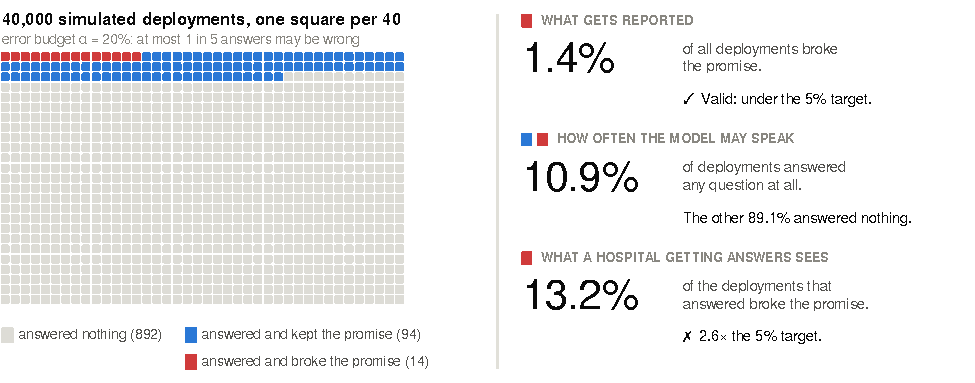
\includegraphics[width=\textwidth]{figs/fig1_overview.pdf}
\caption{\textbf{A valid certificate can be vacuous.} We certify small medical language models at an error budget of 20\% (at most 1 in 5 answers may be wrong) across 40{,}000 simulated deployments. \textbf{Left:} each square stands for 40 deployments (rounded). \textbf{Right:} the usual report counts broken promises over \emph{all} deployments, including the silent ones, and passes. A hospital that gets answers is in one of the deployments that answered. Among those, the promise breaks 2.6 times as often as the limit allows.}
\label{fig:overview}
\end{figure}

\paragraph{Contributions.}
\begin{itemize}[leftmargin=1.4em]
    \item \textbf{Three short results.} A valid certificate promises only $\delta/s$ once it speaks, where $s$ is how often it speaks, and no better bound exists. A certificate needs a minimum number of answers before it may speak. Passing the check is lucky, luck has a ceiling, and rarer passes are luckier.
    \item \textbf{Evidence that all three matter.} On small medical models, the promise breaks in 7.4\% to 39\% of the deployments that speak. At the strictest budget the model never speaks. New questions went worse than the check said in 68\% to 98\% of the deployments that spoke.
    \item \textbf{The price, and a new setting.} The certificate answers 24\% of questions where the same rule without it answers 60\%. Moving to a new benchmark breaks the promise 5.8 times as often.
    \item \textbf{A simple fix.} Every report should say how often the model speaks.
\end{itemize}

%======================================================================
\section{How a safety certificate works}
\label{sec:certificate}
%======================================================================

A model reads a multiple-choice question and gives each option a probability. Its \emph{confidence} is the probability of the option it picks. A certificate sets a \emph{cut-off}. The model answers the questions above the cut-off and says ``I don't know'' to the rest. We use a few plain terms.

\begin{itemize}[leftmargin=1.4em]
    \item \textbf{Error budget $\alpha$.} The largest share of answers that may be wrong. We test 5\%, 10\%, 20\%, 30\%, and 40\%.
    \item \textbf{The promise.} Among the questions the model answers, the error rate stays within $\alpha$.
    \item \textbf{The 5\% limit $\delta$.} A \emph{valid} certificate breaks the promise in at most $\delta = 5\%$ of deployments.
    \item \textbf{Deployment.} One hospital's use of the certificate. It checks the model on 560 practice questions with known answers. Then it uses the model on 140 new questions.
    \item \textbf{Speaks.} The model speaks if the certificate lets it answer at least one question. The \emph{speaking rate} $s$ is the share of deployments in which it speaks.
\end{itemize}

\paragraph{The certificate we test.} We give the certificate every advantage. It splits the practice questions into two halves. The first half proposes cut-offs, from careful (answer few questions) to bold (answer many). The second half checks each cut-off with a standard test \citep{bates2021distribution}. The test asks: is the error rate above this cut-off clearly below $\alpha$? The certificate tries the cut-offs from careful to bold. It stops at the first one that fails and keeps the last one that passed \citep{angelopoulos2022ltt}. If even the most careful cut-off fails, the model stays silent. Appendix~\ref{app:method} gives the details.

%======================================================================
\section{Three simple facts}
\label{sec:theory}
%======================================================================

\paragraph{Setup.} A certificate looks at the practice questions. It returns either a cut-off $\hat\lambda$ or silence. Let $S$ be the event that the model speaks, and let $s = \Pr(S)$. For a cut-off $\lambda$, let $R(\lambda)$ be its true error rate: the share of wrong answers among all future questions it would answer. Silence answers nothing, so its error rate is zero. Let $B$ be the event that the promise breaks: $R(\hat\lambda) > \alpha$. The certificate is \emph{valid} if $\Pr(B) \le \delta$. In our experiments we measure $R$ on the 140 new questions.

\subsection{Fact 1: silence hides failure}

\begin{proposition}[What a valid certificate promises when it speaks]
\label{prop:silence}
For any certificate, $\Pr(B) = s \cdot \Pr(B \mid S)$. So if the certificate is valid,
\begin{equation}
\Pr(B \mid S) \;\le\; \frac{\delta}{s}.
\label{eq:silence}
\end{equation}
No better bound exists. Suppose at least one cut-off keeps the promise and one breaks it. Then for every $s \ge \delta$, some valid certificate speaks with rate $s$ and has $\Pr(B \mid S) = \delta / s$.
\end{proposition}

\begin{proof}
A silent model answers nothing, so it cannot break the promise. So $B$ can only happen when $S$ happens. Then $\Pr(B) = \Pr(B \text{ and } S) = s \cdot \Pr(B \mid S)$. Validity says $\Pr(B) \le \delta$. Dividing by $s$ gives the bound.

For the second part, let $\lambda_{\text{good}}$ keep the promise and $\lambda_{\text{bad}}$ break it. Build a certificate that ignores the data and rolls a die. With probability $\delta$ it uses $\lambda_{\text{bad}}$. With probability $s - \delta$ it uses $\lambda_{\text{good}}$. Otherwise it stays silent. It speaks with probability $s$. It breaks the promise with probability $\delta$, so it is valid. And $\Pr(B \mid S) = \delta / s$.
\end{proof}

In words: validity caps failures across all deployments, and silent deployments never fail. So the less a model speaks, the more of its speech may fail. Table~\ref{tab:room} shows how fast the promise fades.

\begin{table}[h]
\centering
\small
\caption{What a valid certificate (5\% limit) promises once the model speaks.}
\label{tab:room}
\begin{tabular}{lccccc}
\toprule
How often the model speaks, $s$ & 100\% & 50\% & 25\% & 10\% & 5\% or less \\
\midrule
Most failures allowed when it speaks, $\delta/s$ & 5\% & 10\% & 20\% & 50\% & no limit \\
\bottomrule
\end{tabular}
\end{table}

\begin{remark}[Silence buys validity]
\label{rem:buys}
Take any procedure, however bad. Say it breaks the promise with probability $q$ when it speaks. Now let it speak only on a random share $\delta/q$ of deployments. It is now valid. Even a procedure that is \emph{always} wrong is valid if it speaks in only 5\% of deployments. So validity alone cannot tell a careful certificate from a careless one.
\end{remark}

\begin{remark}[One number is not enough]
\label{rem:one}
Say a paper reports only the overall failure rate $b = \Pr(B)$. The failure rate when the model speaks is then $b / s$. Since $s$ can be anything from $b$ to 1, this rate can be anything from $b$ to 100\%. The missing number is $s$.
\end{remark}

\begin{remark}[A screening test]
A certificate works like a screening test for the model, and a pass is a positive result. Validity says that at most 5\% of all deployments end in a false pass. A hospital wants to know what share of \emph{passes} are false. Bayes' rule links the two numbers, just as for a medical test. When true passes are rare, false passes take over.
\end{remark}

\subsection{Fact 2: strict promises force silence}

Proving that something is rare takes many clean examples. If none of 30 patients has a side effect, the true rate could still be 10\%. Medicine calls this the \emph{rule of three}: with no events in $n$ cases, the rate could still be about $3/n$ \citep{hanley1983nothing}. The same rule limits a certificate.

\begin{proposition}[A floor on what can be proved]
\label{prop:three}
Suppose the check is a valid test: if a cut-off's true error is $\alpha$ or more, the check passes it with probability at most $\delta$. Suppose also that fewer errors never hurt: if the check passes a cut-off with $k$ errors, it also passes it with fewer. Then the check can only pass a cut-off that answers at least
\begin{equation}
n_0 \;=\; \frac{\ln(1/\delta)}{\ln\!\big(1/(1-\alpha)\big)} \;\approx\; \frac{3}{\alpha}
\label{eq:three}
\end{equation}
practice questions. The approximation holds for small $\alpha$ and $\delta = 5\%$.
\end{proposition}

\begin{proof}
Take a cut-off whose true error is exactly $\alpha$. Say it answers $n$ practice questions. If the check can pass it at all, it passes it when there are zero errors, because fewer errors never hurt. Zero errors happen with probability $(1-\alpha)^n$. So the check passes with probability at least $(1-\alpha)^n$. Validity needs this to be at most $\delta$. Solving $(1-\alpha)^n \le \delta$ for $n$ gives $n \ge n_0$. For the approximation, note that $\ln 20 \approx 3$ and that $\ln(1/(1-\alpha)) \approx \alpha$ when $\alpha$ is small.
\end{proof}

The floor does not depend on the model at all. It is the cost of proof. At our budgets of 5\%, 10\%, 20\%, 30\%, and 40\%, the floor is 59, 29, 14, 9, and 6 answers. Our certificate checks up to 20 cut-offs, so it uses the stricter limit $\delta/20$. Its floor is 117, 57, 27, 17, and 12 answers (Appendix~\ref{app:method}).

\begin{corollary}[Forced silence]
\label{cor:forced}
Suppose every cut-off the certificate may use has a true error above $\alpha$. Then each time the model speaks, it breaks the promise: $\Pr(B \mid S) = 1$. Validity then forces $s \le \delta$.
\end{corollary}

\begin{proof}
Each time the model speaks, it uses a cut-off with error above $\alpha$. So $S$ implies $B$, and $s = \Pr(S) \le \Pr(B) \le \delta$.
\end{proof}

Put the two results together. Proposition~\ref{prop:three} says the certificate may only use cut-offs that answer many questions. If no cut-off can answer that many questions safely, Corollary~\ref{cor:forced} applies. So a strict budget on a weak model ends in silence, or in broken promises.

\subsection{Fact 3: passing is luck}

\paragraph{Setup.} Fix one cut-off, chosen on the first half of the practice questions. It answers $n$ questions in the second half. Let $R$ be its true error, $\hat R$ its error on those $n$ questions, and $\Rnew$ its error on new questions. Let ``pass'' be any event decided by the second half, with probability $p$ given $n$. The \emph{luck} of a pass is
\[
L \;=\; \E\big[\, \Rnew - \hat R \;\big|\; \text{pass} \,\big].
\]
It measures how much worse new questions go than the practice questions said.

\begin{proposition}[Passing is luck, and luck has a ceiling]
\label{prop:luck}
\leavevmode
\begin{enumerate}[label=(\alph*),leftmargin=1.6em]
    \item \textbf{Luck has a ceiling.} For any rule that decides a pass, $L \le \sqrt{\ln(1/p) \,/\, (2n)}$.
    \item \textbf{A threshold check is always lucky.} If the check passes exactly when $\hat R \le c$, then $L \ge 0$.
    \item \textbf{Rarer passes are luckier.} Suppose also that $\hat R = R + \sigma Z$, where the shape of the noise $Z$ does not depend on $R$. Then $L = \sigma\, g(p)$ for a function $g$ that falls as $p$ grows and reaches 0 at $p = 1$. For bell-shaped (Gaussian) noise, $g(p) = \varphi(\Phi^{-1}(p))/p$. So $g(50\%) \approx 0.80$, $g(10\%) \approx 1.75$, and $g(1\%) \approx 2.67$.
\end{enumerate}
\end{proposition}

The proof rests on two short lemmas.

\begin{lemma}[Rare events can only be so lucky]
\label{lem:ceiling}
Let $X$ have mean zero, and suppose $\E[e^{\theta X}] \le e^{\theta^2\sigma^2/2}$ for every $\theta$. Then for any event $A$ with $\Pr(A) = p > 0$,
\[
\E[X \mid A] \;\le\; \sigma\sqrt{2\ln(1/p)}.
\]
\end{lemma}

\begin{proof}
Take $\theta > 0$. Jensen's inequality gives $e^{\theta\E[X \mid A]} \le \E[e^{\theta X} \mid A]$. The right side is at most $\E[e^{\theta X}]/p$, because $A$ holds only a share $p$ of the time. That is at most $e^{\theta^2\sigma^2/2}/p$. Take logs and divide by $\theta$: $\E[X \mid A] \le \theta\sigma^2/2 + \ln(1/p)/\theta$. Choosing $\theta = \sqrt{2\ln(1/p)}/\sigma$ gives the result.
\end{proof}

\begin{lemma}[The low end sits below the mean]
\label{lem:tail}
For any $Z$ with a finite mean, $\E[Z \mid Z \le t] \le \E[Z]$. Also, $\E[Z \mid Z \le t]$ grows with $t$.
\end{lemma}

\begin{proof}
Split $Z$ at $t$. The mean $\E[Z]$ is a weighted average of $\E[Z \mid Z \le t]$, which is at most $t$, and $\E[Z \mid Z > t]$, which is above $t$. So the first is at most the average. Now take $t < t'$. The mean $\E[Z \mid Z \le t']$ is a weighted average of $\E[Z \mid Z \le t]$ and $\E[Z \mid t < Z \le t']$. The second is above $t$, which is above the first. So moving from $t$ to $t'$ can only raise the mean.
\end{proof}

\begin{proof}[Proof of Proposition~\ref{prop:luck}]
New questions are independent of the practice questions, and $\E[\Rnew] = R$. So $L = \E[R - \hat R \mid \text{pass}]$.

\emph{Part (a).} $\hat R$ is an average of $n$ independent errors, each 0 or 1, with mean $R$. By Hoeffding's lemma \citep{hoeffding1963probability}, $X = R - \hat R$ meets Lemma~\ref{lem:ceiling} with $\sigma = 1/(2\sqrt n)$. Then $\sigma\sqrt{2\ln(1/p)} = \sqrt{\ln(1/p)/(2n)}$.

\emph{Part (b).} Apply Lemma~\ref{lem:tail} with $Z = \hat R$ and $t = c$. This gives $\E[\hat R \mid \text{pass}] \le \E[\hat R] = R$.

\emph{Part (c).} A pass means $Z \le t$, where $t = (c - R)/\sigma$. Its probability is $p = \Pr(Z \le t)$, so $t$ is the $p$-th quantile of $Z$. Then $L = -\sigma\,\E[Z \mid Z \le t]$ depends on $p$ alone. By Lemma~\ref{lem:tail}, it falls as $p$ grows. At $p = 1$ it equals $-\sigma\E[Z] = 0$. For Gaussian $Z$, $\E[Z \mid Z \le t] = -\varphi(t)/\Phi(t)$.
\end{proof}

\begin{remark}[The ceiling is tight]
For Gaussian noise, $g(p)/\sqrt{2\ln(1/p)} \to 1$ as $p \to 0$ (Appendix~\ref{app:proofs}). So when passes are rare, a plain threshold check is about as lucky as any rule can be.
\end{remark}

\begin{remark}[Many cut-offs]
\label{rem:many}
Our certificate tries up to $G = 20$ cut-offs and uses one. The same proof, applied to the largest of the $G$ gaps, gives the ceiling $\sqrt{\ln(G/p)/(2n)}$, with $n$ the smallest answer count (Appendix~\ref{app:proofs}). Trying more cut-offs buys more luck, but only slowly.
\end{remark}

\begin{remark}[What the ceiling means]
A cut-off that answers 30 questions and passes once in 100 tries can look up to 28 points better than it is. With 300 answers, the ceiling drops to 9 points. More answers shrink the luck. But rare passes always deserve suspicion.
\end{remark}

\subsection{What the facts predict}
\label{sec:predictions}

The three facts make four predictions that we can test.
\begin{enumerate}[label=\textbf{P\arabic*.},leftmargin=2.2em]
    \item The promise holds overall, yet breaks often when the model speaks. \hfill (Proposition~\ref{prop:silence})
    \item At strict budgets the model stays silent. \hfill (Proposition~\ref{prop:three}, Corollary~\ref{cor:forced})
    \item When the model speaks, new questions go worse than the check said. \hfill (Proposition~\ref{prop:luck}b)
    \item This gap is largest where passing is rarest. \hfill (Proposition~\ref{prop:luck}c)
\end{enumerate}

%======================================================================
\section{Testing the facts on small medical models}
\label{sec:experiments}
%======================================================================

\paragraph{Setup.} We use 700 questions from each of four public medical benchmarks: MedMCQA \citep{pal2022medmcqa}, MedQA \citep{jin2021disease}, the medical and biology parts of MMLU \citep{hendrycks2021mmlu}, and PubMedQA \citep{jin2019pubmedqa}. We test ten configurations of eight open models: Qwen2.5 at 0.5B, 1.5B, 3B, and 7B \citep{qwen2024qwen25}, SmolLM2-1.7B \citep{allal2025smollm2}, Granite-3.1-2B \citep{granite2024}, Mistral-7B \citep{jiang2023mistral}, and the medical model BioMistral-7B \citep{labrak2024biomistral}. The 7B models run in 4-bit form \citep{dettmers2023qlora}. Qwen2.5 1.5B and 3B run in both 16-bit and 4-bit form as a check. For each model and benchmark we simulate 1{,}000 deployments. Each has its own 560 practice questions and 140 new questions. That gives 40{,}000 deployments in all. Everything ran on one 16\,GB graphics card.

\subsection{The promise holds by staying silent (P1, P2)}

The certificate keeps its promise at every budget (Figure~\ref{fig:within}a). The share of deployments that broke it is 0.0\%, 0.2\%, 1.4\%, 2.5\%, and 3.0\% as the budget grows from 5\% to 40\%. Every 95\% interval stays below 5\%.

But the model rarely speaks (Figure~\ref{fig:within}b). At a 5\% budget it speaks in none of the 40{,}000 deployments. At 10\% it speaks in 0.5\%, at 20\% in 10.9\%, at 30\% in 25.8\%, and at 40\% in 40.5\%. Even at the loosest budget, 59.5\% of deployments never answer.

Fact 2 explains the silence at strict budgets (P2). At a 5\% budget, the best possible cut-off answers only 5.3\% of questions. That is about 15 of the 280 questions the check sees. Even the most lenient valid check would need 59 (Proposition~\ref{prop:three}), and ours needs 117. So any time the model spoke would be a mistake (Corollary~\ref{cor:forced}). In 40{,}000 deployments, it never spoke. At 10\%, the best cut-off answers about 29 questions, against a floor of 57. The model speaks in only 0.5\% of deployments. That is below $\delta$, so by Proposition~\ref{prop:silence} its promise means nothing when it speaks.

\begin{figure}[t]
\centering
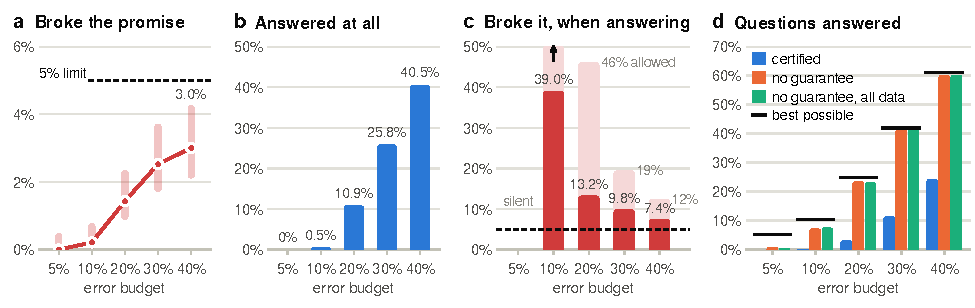
\includegraphics[width=\textwidth]{figs/fig2_within.pdf}
\caption{\textbf{The promise holds by staying silent, and breaks often when the model speaks.} 40{,}000 deployments per budget. \textbf{(a)} Share of all deployments that broke the promise, with 95\% intervals. It stays under the 5\% limit (dashed). \textbf{(b)} Share of deployments where the model answered at least one question. \textbf{(c)} Share of answering deployments that broke the promise (dark), and the most that Proposition~\ref{prop:silence} allows, $\delta/s$ (light). The arrow means no limit. \textbf{(d)} Share of new questions answered by the certificate, by the same rule without a guarantee, by that rule with all the data, and by the best possible cut-off (black line).}
\label{fig:within}
\end{figure}

\subsection{When the model speaks, the promise often breaks (P1)}

A hospital only sees the deployments that answer. Among those, the promise broke in 39.0\%, 13.2\%, 9.8\%, and 7.4\% of deployments at budgets of 10\% to 40\% (Figure~\ref{fig:within}c). Every one is above 5\%. Every one is also within the limit $\delta/s$ from Proposition~\ref{prop:silence}: no limit, 46\%, 19\%, and 12\%. So this is not a flaw in our certificate. The guarantee allows it.

\subsection{Passing is luck (P3, P4)}

For each deployment that spoke, we compare two error rates at the chosen cut-off. One is the rate the check saw on practice questions. The other is the rate on new questions. New questions went worse by 11.4, 17.6, 13.7, and 11.7 percentage points at budgets of 10\% to 40\% (Figure~\ref{fig:luck}a). Every 95\% interval excludes zero. A few outliers do not drive this. New questions went worse in 98\%, 88\%, 74\%, and 68\% of these deployments, where chance would give 50\% (Figure~\ref{fig:luck}b). This confirms P3.

\begin{figure}[t]
\centering
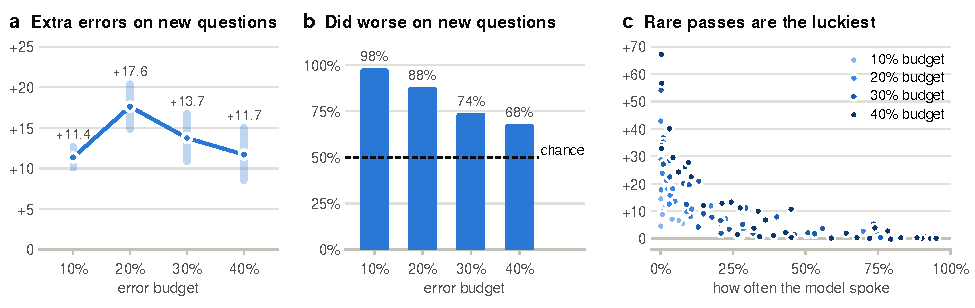
\includegraphics[width=\textwidth]{figs/fig3_luck.pdf}
\caption{\textbf{Passing the check is luck.} Only deployments where the model spoke. \textbf{(a)} Error on new questions minus error on practice questions, in percentage points, with 95\% intervals. \textbf{(b)} Share of these deployments where new questions went worse. The dashed line is chance. \textbf{(c)} The same gap for each model, benchmark, and budget, against how often that combination spoke. Proposition~\ref{prop:luck}c predicts the downward trend.}
\label{fig:luck}
\end{figure}

Figure~\ref{fig:luck}c tests P4. Each dot is one model, benchmark, and budget. The gap is positive for 116 of the 117 dots. It falls steadily as speaking becomes common. The rank correlation is $-0.86$ overall, and between $-0.90$ and $-0.96$ within each budget from 20\% to 40\%. When a combination speaks less than 5\% of the time, the median gap is 26 points. When it speaks more than half the time, the median gap is 0.4 points. Rare passes are the luckiest, as Proposition~\ref{prop:luck} predicts.

\subsection{The price of silence}

Silence costs answers (Figure~\ref{fig:within}d). At a 40\% budget the certificate answers 24.3\% of new questions. The same rule without the guarantee answers 60.1\%. With all the data, it answers 60.2\%. The best possible cut-off answers 61.1\%. So the rule without a guarantee gets 98\% of the way to the best possible, and the certificate gets 40\%. More data is not the fix. It changes coverage by at most 0.4 points at any budget. The guarantee itself takes the answers.

\subsection{A new benchmark breaks the promise}

A hospital rarely gets questions exactly like its practice set. So we also check the model on one benchmark and use it on another. This covers 12 benchmark pairs and 36{,}000 deployments. As a control, the same cut-off is also used on new questions from the practice benchmark. Both arms speak in the same deployments, so the only difference is the switch.

\begin{figure}[t]
\centering
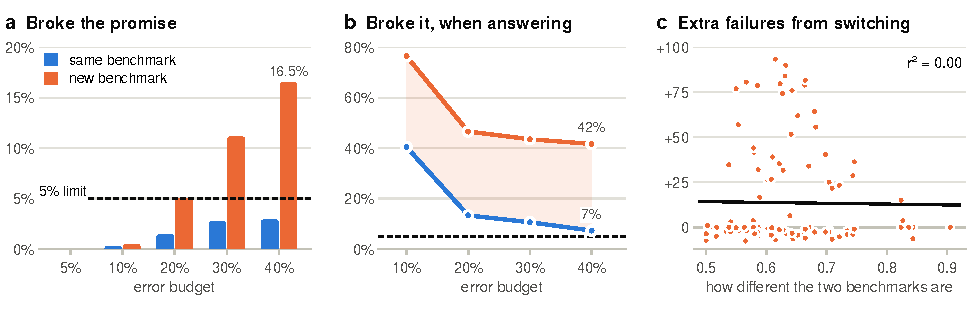
\includegraphics[width=\textwidth]{figs/fig4_transport.pdf}
\caption{\textbf{A new benchmark breaks the promise.} 36{,}000 deployments per budget. \textbf{(a)} Share of all deployments that broke the promise, on a new benchmark (orange) or on the practice benchmark (blue). \textbf{(b)} The same, among deployments that answered. \textbf{(c)} For each model and benchmark pair at a 40\% budget: extra broken promises from switching, in points, against how easily a classifier tells the two benchmarks apart (0.5 means it cannot).}
\label{fig:transport}
\end{figure}

Switching breaks the promise in 5.0\%, 11.1\%, and 16.5\% of all deployments at budgets of 20\%, 30\%, and 40\% (Figure~\ref{fig:transport}a). The control breaks it in 1.4\%, 2.7\%, and 2.9\%. At 40\%, switching breaks the promise 5.8 times as often. Among deployments that answered, the rates are 42\% and 7\% (Figure~\ref{fig:transport}b). The control's 7.2\% matches the 7.4\% from before, as it should.

The standard fix reweights the practice questions to look like the new benchmark \citep{tibshirani2019conformal}. It never let the model speak, in any of the 36{,}000 deployments. It is valid for the same reason a silent model is safe. Nor can a hospital tell in advance which switches are risky. How easily a classifier tells two benchmarks apart explains none of the damage ($r^2 = 0.00$; Figure~\ref{fig:transport}c).

%======================================================================
\section{What to report, and what comes next}
\label{sec:report}
%======================================================================

\begin{plainbox}{What every report on a safety certificate should include}
\begin{enumerate}[leftmargin=1.3em,label=\textbf{\arabic*.}]
    \item \textbf{How often the model speaks.} Without it, the failure rate means little (Remark~\ref{rem:one}).
    \item \textbf{The failure rate when the model speaks.} It is what a hospital lives with. Proposition~\ref{prop:silence} caps it at $\delta/s$.
    \item \textbf{How many questions it answers}, next to a rule without a guarantee and the best possible cut-off.
    \item \textbf{A matched control} for any test on new data, so luck is not mistaken for a real difference.
\end{enumerate}
\end{plainbox}

\paragraph{A promise for when the model speaks.} A hospital wants a promise that holds when the model speaks. Methods that correct for a selection step exist for related problems \citep{jin2023selection,bao2024selective}. Proposition~\ref{prop:silence} shows the cost. A promise of $\delta$ when speaking needs a certificate that is valid at $\delta s$. That is stricter still when $s$ is small.

\paragraph{Beyond medicine.} Nothing in Section~\ref{sec:theory} is about medicine. The three facts apply to any system that may decline to act: a chatbot that refuses, a triage tool that defers to a doctor, a car that hands control back to its driver. Each such system should report how often it acts.

%======================================================================
\section{Related work}
%======================================================================

\paragraph{Answering only when confident.} Selective prediction lets a model skip hard inputs \citep{el2010foundations,geifman2017selective}. Risk control turns this into a guarantee with no assumptions about the model \citep{bates2021distribution,angelopoulos2022ltt}. It builds on conformal prediction \citep{vovk2005algorithmic,angelopoulos2023conformal}. It has been applied to language models for multiple choice \citep{kumar2023conformal}, text generation \citep{quach2024conformal}, and factual claims \citep{mohri2024factuality}. These works check whether the guarantee holds. We show that this check means little without the speaking rate.

\paragraph{Limits of such guarantees.} These guarantees hold on average. Other kinds of validity must be targeted on purpose \citep{vovk2012conditional}. Exact validity for each input is impossible without assumptions \citep{barber2021limits}. Coverage after a selection step needs its own correction \citep{jin2023selection,bao2024selective}. Proposition~\ref{prop:silence} is a simple case of the same idea. Proposition~\ref{prop:luck} is a form of the winner's curse, well known in genetics \citep{zollner2007overcoming}. Our contribution is to state these facts for certificates that may stay silent, and to show that their effects are large in practice.

\paragraph{Confidence of language models.} Language models are often overconfident \citep{guo2017calibration,desai2020calibration,kadavath2022know}, more so on unfamiliar data \citep{ovadia2019trust}. They also change answers when the options are reordered \citep{zheng2024selectors}. Medical models are usually judged on accuracy alone \citep{singhal2023medpalm}. Our small models show the same problems (Appendix~\ref{app:signal}).

%======================================================================
\section{Conclusion}
%======================================================================

The world is building small AI models that hospitals can run themselves. Safety certificates are a natural way to make them safe. We proved three facts. Silence hides failure. Strict promises force silence. Passing is luck. On small medical models, all three show up clearly. The certificates keep their promise, but mostly by staying silent. When they speak, they break it 1.5 to 8 times as often as the 5\% limit. Certification is still useful. But a failure rate without a speaking rate is not a safety claim. Before asking how often a model is wrong, ask how often it spoke.

\FloatBarrier
\bibliographystyle{plainnat}
\bibliography{refs}

%======================================================================
\appendix
\clearpage
\section*{Appendix}
%======================================================================

\section{The certificate in full}
\label{app:method}

\paragraph{Notation.} Let $\lambda$ be a confidence cut-off. A question counts as an error if the model answers it (its confidence is above $\lambda$) and gets it wrong. The \emph{selective risk} at $\lambda$ is the error rate among answered questions.

\paragraph{Cut-offs are listed by answer count.} Suppose cut-offs were spread evenly on the confidence scale. Then the highest ones would answer only a handful of questions. No test can prove a low error rate from a handful of answers. So the certificate would stop at its first step for no good reason. We therefore list cut-offs by how many questions they answer. The list starts at the \emph{floor}, the smallest count that could pass with zero errors:
\begin{equation}
n_{\min}(\alpha) \;=\; \min \Big\{ n \;:\; p_{\mathrm{HB}}(0, n, \alpha) \;\le\; \delta / G \Big\}.
\end{equation}
Here $p_{\mathrm{HB}}$ is the Hoeffding--Bentkus p-value \citep{bates2021distribution} and $G = 20$ is the number of cut-offs. With zero errors, $p_{\mathrm{HB}}(0, n, \alpha) = (1-\alpha)^n$. So the floor is Proposition~\ref{prop:three} with $\delta/G$ in place of $\delta$. The list runs from the floor up to the size of the first half. Table~\ref{tab:feasibility} gives the floors. Every budget has a full list at our sample size. So the silence at a 5\% budget comes from the data, not from an empty list.

\begin{table}[H]
\centering
\small
\caption{The floor: the fewest answers that could pass the check with zero errors. The first half of the practice questions holds 280 questions.}
\label{tab:feasibility}
\begin{tabular}{lccccc}
\toprule
Error budget $\alpha$ & 5\% & 10\% & 20\% & 30\% & 40\% \\
\midrule
Floor, one test ($\delta = 5\%$) & 59 & 29 & 14 & 9 & 6 \\
Floor, 20 cut-offs ($\delta/20$) & 117 & 57 & 27 & 17 & 12 \\
Cut-offs on the list & 20 & 20 & 20 & 20 & 20 \\
\bottomrule
\end{tabular}
\end{table}

\paragraph{Why the practice questions are split.} The test needs the cut-off to be fixed before it sees the questions used to test it. A cut-off listed by answer count is the $k$-th highest confidence among the practice questions. If we tested it on the same questions, we would test it on its own best cases. So we split the 560 practice questions in two. The first half (280) turns each count $k$ into a cut-off $\hat\lambda_k$. The second half (280) measures the error at $\hat\lambda_k$ and computes the p-value. The cut-off does not depend on the second half, so the test is valid.

\paragraph{The order of testing.} We test the cut-offs from the floor upward and stop at the first one that fails. This fixed-order method keeps the chance of any false pass within $\delta$ for any order fixed in advance \citep{angelopoulos2022ltt}. So validity does not need the error to grow with the number of answers. The certificate returns the boldest cut-off that passed, or silence. As extra checks, we also ran a Bonferroni correction over all 20 cut-offs and an exact binomial p-value. Validity holds under both.

\paragraph{What we report.} A deployment \emph{breaks the promise} if its error on the 140 new questions is above $\alpha$. Silent deployments count as keeping the promise, since that is how the guarantee counts them. The \emph{speaking rate} is the share of deployments with a cut-off. The failure rate when speaking is the ratio of the two pooled counts (Table~\ref{tab:counts}). Rates get 95\% Wilson intervals. Differences get 95\% bootstrap intervals.

\paragraph{Reference rules.} \emph{No guarantee} picks the boldest cut-off whose practice error is at most $\alpha$, with no test. \emph{All data} does the same with the cut-off chosen on the whole benchmark. This mimics unlimited practice data. \emph{Best possible} picks the cut-off with the most answers whose error on the new questions is at most $\alpha$, using their answers. The gap from the certificate to \emph{no guarantee} is the price of the guarantee. The gap from \emph{no guarantee} to \emph{all data} is the price of limited data.

\paragraph{New benchmarks.} The plain arm uses the cut-off on another benchmark. The control uses the same cut-off on new questions from the practice benchmark, cut down to the same number of answers. The reweighted arm weights each practice question by an estimated likelihood ratio. The ratio comes from a classifier that tells the two benchmarks apart. Weights are clipped at 2, 5, or 20. The arm uses an empirical Bernstein bound, which adapts to the spread of the weighted errors.

\paragraph{Plan and compute.} Cut-offs, reference rules, and tests were fixed before we saw results. Confidence is the softmax over the option letters' next-token scores, with no temperature scaling. Every question was scored by every configuration in the original and a shuffled option order. That is 56{,}000 scored cells, which took 3.3 hours on one NVIDIA T4. All statistics run in 14 minutes on a CPU from cached scores.

\section{More on the proofs}
\label{app:proofs}

\paragraph{Many cut-offs (Remark~\ref{rem:many}).} The certificate fixes $G$ cut-offs $\lambda_1, \dots, \lambda_G$ on the first half. It then picks one, $\lambda_J$, using the second half. Let $X_j = R(\lambda_j) - \hat R_j$, where cut-off $j$ answers $n_j$ questions in the second half. Each $X_j$ has mean zero. By Hoeffding's lemma, each meets Lemma~\ref{lem:ceiling} with $\sigma_j = 1/(2\sqrt{n_j}) \le \sigma = 1/(2\sqrt{n_{\min}})$, where $n_{\min} = \min_j n_j$. New questions are independent of the second half, and their error has mean $R(\lambda_j)$ given $J = j$. So the luck of a pass with probability $p$ is $L = \E[X_J \mid \text{pass}] \le \E[\max_j X_j \mid \text{pass}]$. For $\theta > 0$, Jensen's inequality and $e^{\theta\max_j X_j} \le \sum_j e^{\theta X_j}$ give
\[
e^{\theta\,\E[\max_j X_j \mid \text{pass}]} \;\le\; \frac{\E\big[\sum_j e^{\theta X_j}\big]}{p} \;\le\; \frac{G\, e^{\theta^2\sigma^2/2}}{p}.
\]
Taking logs and choosing $\theta$ as in Lemma~\ref{lem:ceiling} gives $L \le \sigma\sqrt{2\ln(G/p)} = \sqrt{\ln(G/p)/(2n_{\min})}$.

\paragraph{Why a threshold check is nearly the luckiest rule.} Take Gaussian $Z$ and $t = \Phi^{-1}(p)$. As $p \to 0$, the Mills ratio gives $\varphi(t)/\Phi(t) = |t|\,(1 + o(1))$. Also $|\Phi^{-1}(p)| = \sqrt{2\ln(1/p)}\,(1 + o(1))$. So $g(p) / \sqrt{2\ln(1/p)} \to 1$, and the ceiling in Proposition~\ref{prop:luck}a is tight as $p \to 0$.

\paragraph{The rule of three for our test.} The Hoeffding--Bentkus p-value grows with the number of errors. So our check meets the ``fewer errors never hurt'' condition of Proposition~\ref{prop:three}. With zero errors its p-value is exactly $(1-\alpha)^n$. So our floor meets the bound of Proposition~\ref{prop:three} exactly, after rounding $n$ up.

\paragraph{What the theory assumes.} Proposition~\ref{prop:silence} and Corollary~\ref{cor:forced} assume nothing beyond validity. Proposition~\ref{prop:luck}a and~b assume only that the cut-off is fixed before the second half is seen. Our split ensures this. Proposition~\ref{prop:luck}c also assumes the noise has the same shape at every true error. For a binomial count this holds only roughly. So we test~(c) on data rather than rely on it.

\section{Exact counts}
\label{app:counts}

\begin{table}[H]
\centering
\small
\caption{Counts behind Figures~\ref{fig:overview} and~\ref{fig:within}. Each budget has 40{,}000 deployments (10 configurations $\times$ 4 benchmarks $\times$ 1{,}000). The limit is $\delta/s$ (Proposition~\ref{prop:silence}).}
\label{tab:counts}
\begin{tabular}{lrrrrrr}
\toprule
Budget $\alpha$ & Spoke & Broke & Broke (all) & Speaking rate & Broke (spoke) & Limit \\
\midrule
5\%  & 0      & 0     & 0.00\% & 0.00\%  & --      & --      \\
10\% & 218    & 85    & 0.21\% & 0.55\%  & 39.0\%  & none    \\
20\% & 4{,}340  & 573   & 1.43\% & 10.85\% & 13.2\%  & 46.1\%  \\
30\% & 10{,}314 & 1{,}011 & 2.53\% & 25.79\% & 9.8\%   & 19.4\%  \\
40\% & 16{,}200 & 1{,}201 & 3.00\% & 40.50\% & 7.4\%   & 12.3\%  \\
\bottomrule
\end{tabular}
\end{table}

\begin{table}[H]
\centering
\small
\caption{Counts behind Figure~\ref{fig:transport}. Each budget has 36{,}000 deployments (10 configurations $\times$ 12 benchmark pairs $\times$ 300). Both arms speak in the same deployments.}
\label{tab:transport}
\begin{tabular}{lrrrrrr}
\toprule
 & & \multicolumn{2}{c}{Broke the promise} & \multicolumn{2}{c}{Broke (share of spoke)} & \\
\cmidrule(lr){3-4}\cmidrule(lr){5-6}
Budget $\alpha$ & Spoke & New & Same & New & Same & Ratio \\
\midrule
10\% & 208     & 159   & 84    & 76.4\% & 40.4\% & 1.9 \\
20\% & 3{,}848  & 1{,}791 & 511   & 46.5\% & 13.3\% & 3.5 \\
30\% & 9{,}185  & 3{,}995 & 970   & 43.5\% & 10.6\% & 4.1 \\
40\% & 14{,}261 & 5{,}935 & 1{,}032 & 41.6\% & 7.2\%  & 5.8 \\
\bottomrule
\end{tabular}
\end{table}

\begin{table}[H]
\centering
\small
\caption{Share of new questions answered, behind Figure~\ref{fig:within}d.}
\label{tab:coverage}
\begin{tabular}{lccccc}
\toprule
Budget $\alpha$ & 5\% & 10\% & 20\% & 30\% & 40\% \\
\midrule
Certificate & 0.0\% & 0.1\% & 3.1\% & 11.4\% & 24.3\% \\
No guarantee & 0.9\% & 7.1\% & 23.5\% & 41.4\% & 60.1\% \\
No guarantee, all data & 0.5\% & 7.5\% & 23.1\% & 41.5\% & 60.2\% \\
Best possible & 5.3\% & 10.3\% & 24.9\% & 42.0\% & 61.1\% \\
\bottomrule
\end{tabular}
\end{table}

\section{Accuracy by model and benchmark}

Table~\ref{tab:accuracy} gives accuracy for every configuration and benchmark, with 95\% Wilson intervals. It also gives accuracy and answer agreement when the options are shuffled. Mean accuracy is 0.531. Mean agreement under shuffling is 0.727, ranging from 0.539 to 0.949.

{\small
\begin{longtable}{llcccc}
\caption{Accuracy by configuration and benchmark ($n = 700$ questions per cell), with accuracy and answer agreement under shuffled options.}
\label{tab:accuracy} \\
\toprule
Model & Benchmark & Accuracy & 95\% CI & Shuffled accuracy & Agreement \\
\midrule
\endfirsthead
\toprule
Model & Benchmark & Accuracy & 95\% CI & Shuffled accuracy & Agreement \\
\midrule
\endhead
\bottomrule
\endfoot
BioMistral-7B (nf4) & MMLU & 0.576 & {[0.539, 0.612]} & 0.540 & 0.659 \\
BioMistral-7B (nf4) & MedMCQA & 0.421 & {[0.385, 0.458]} & 0.407 & 0.563 \\
BioMistral-7B (nf4) & MedQA & 0.439 & {[0.402, 0.476]} & 0.456 & 0.663 \\
BioMistral-7B (nf4) & PubMedQA & 0.433 & {[0.397, 0.470]} & 0.559 & 0.606 \\
\midrule
Granite-3.1-2B (fp16) & MMLU & 0.583 & {[0.546, 0.619]} & 0.557 & 0.653 \\
Granite-3.1-2B (fp16) & MedMCQA & 0.371 & {[0.336, 0.408]} & 0.394 & 0.539 \\
Granite-3.1-2B (fp16) & MedQA & 0.401 & {[0.366, 0.438]} & 0.403 & 0.596 \\
Granite-3.1-2B (fp16) & PubMedQA & 0.599 & {[0.562, 0.634]} & 0.631 & 0.763 \\
\midrule
Mistral-7B-v0.3 (nf4) & MMLU & 0.601 & {[0.565, 0.637]} & 0.616 & 0.740 \\
Mistral-7B-v0.3 (nf4) & MedMCQA & 0.497 & {[0.460, 0.534]} & 0.480 & 0.671 \\
Mistral-7B-v0.3 (nf4) & MedQA & 0.530 & {[0.493, 0.567]} & 0.526 & 0.719 \\
Mistral-7B-v0.3 (nf4) & PubMedQA & 0.533 & {[0.496, 0.570]} & 0.650 & 0.754 \\
\midrule
Qwen2.5-0.5B (fp16) & MMLU & 0.444 & {[0.408, 0.481]} & 0.463 & 0.611 \\
Qwen2.5-0.5B (fp16) & MedMCQA & 0.361 & {[0.327, 0.398]} & 0.324 & 0.560 \\
Qwen2.5-0.5B (fp16) & MedQA & 0.350 & {[0.316, 0.386]} & 0.343 & 0.577 \\
Qwen2.5-0.5B (fp16) & PubMedQA & 0.591 & {[0.555, 0.627]} & 0.573 & 0.949 \\
\midrule
Qwen2.5-1.5B (fp16) & MMLU & 0.621 & {[0.585, 0.657]} & 0.619 & 0.799 \\
Qwen2.5-1.5B (fp16) & MedMCQA & 0.476 & {[0.439, 0.513]} & 0.429 & 0.694 \\
Qwen2.5-1.5B (fp16) & MedQA & 0.490 & {[0.453, 0.527]} & 0.493 & 0.793 \\
Qwen2.5-1.5B (fp16) & PubMedQA & 0.651 & {[0.615, 0.686]} & 0.679 & 0.851 \\
\midrule
Qwen2.5-1.5B (nf4) & MMLU & 0.599 & {[0.562, 0.634]} & 0.597 & 0.767 \\
Qwen2.5-1.5B (nf4) & MedMCQA & 0.450 & {[0.414, 0.487]} & 0.401 & 0.669 \\
Qwen2.5-1.5B (nf4) & MedQA & 0.437 & {[0.401, 0.474]} & 0.453 & 0.756 \\
Qwen2.5-1.5B (nf4) & PubMedQA & 0.669 & {[0.633, 0.702]} & 0.676 & 0.869 \\
\midrule
Qwen2.5-3B (fp16) & MMLU & 0.693 & {[0.658, 0.726]} & 0.699 & 0.870 \\
Qwen2.5-3B (fp16) & MedMCQA & 0.497 & {[0.460, 0.534]} & 0.471 & 0.723 \\
Qwen2.5-3B (fp16) & MedQA & 0.513 & {[0.476, 0.550]} & 0.497 & 0.781 \\
Qwen2.5-3B (fp16) & PubMedQA & 0.704 & {[0.669, 0.737]} & 0.669 & 0.881 \\
\midrule
Qwen2.5-3B (nf4) & MMLU & 0.674 & {[0.639, 0.708]} & 0.676 & 0.821 \\
Qwen2.5-3B (nf4) & MedMCQA & 0.487 & {[0.450, 0.524]} & 0.496 & 0.740 \\
Qwen2.5-3B (nf4) & MedQA & 0.491 & {[0.455, 0.528]} & 0.503 & 0.776 \\
Qwen2.5-3B (nf4) & PubMedQA & 0.696 & {[0.661, 0.729]} & 0.673 & 0.900 \\
\midrule
Qwen2.5-7B (nf4) & MMLU & 0.760 & {[0.727, 0.790]} & 0.741 & 0.881 \\
Qwen2.5-7B (nf4) & MedMCQA & 0.563 & {[0.526, 0.599]} & 0.560 & 0.791 \\
Qwen2.5-7B (nf4) & MedQA & 0.589 & {[0.552, 0.624]} & 0.607 & 0.794 \\
Qwen2.5-7B (nf4) & PubMedQA & 0.726 & {[0.691, 0.757]} & 0.720 & 0.946 \\
\midrule
SmolLM2-1.7B (fp16) & MMLU & 0.487 & {[0.450, 0.524]} & 0.503 & 0.623 \\
SmolLM2-1.7B (fp16) & MedMCQA & 0.357 & {[0.323, 0.393]} & 0.324 & 0.570 \\
SmolLM2-1.7B (fp16) & MedQA & 0.367 & {[0.332, 0.403]} & 0.354 & 0.587 \\
SmolLM2-1.7B (fp16) & PubMedQA & 0.494 & {[0.457, 0.531]} & 0.559 & 0.583 \\
\end{longtable}}

\section{The confidence signal}
\label{app:signal}

Every certificate rests on the model's confidence (Figure~\ref{fig:models}). Confidence carries real information. Every configuration ranks right answers above wrong ones better than chance. The area under the risk--coverage curve (lower is better) runs from 0.192 for Qwen2.5-7B, against 0.342 for random order, to 0.460 for SmolLM2-1.7B, against 0.573. But all 40 model and benchmark pairs are overconfident. The mean calibration error is 0.252, and mean confidence beats accuracy by the same margin. Shuffling the answer options changes the model's answer on 27.3\% of questions on average. In the worst case (Granite-3.1-2B on MedMCQA) it changes 46.1\%. Any cut-off on this signal inherits that instability.

\begin{figure}[H]
\centering
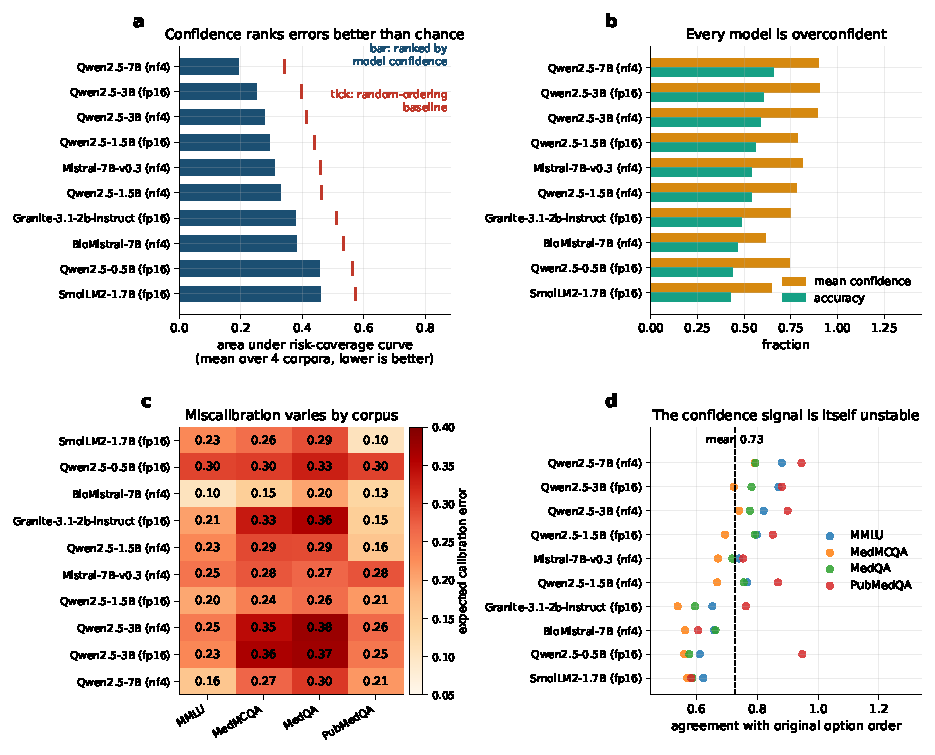
\includegraphics[width=0.95\textwidth]{figs/fig5_models.pdf}
\caption{\textbf{Confidence is informative, overconfident, and unstable.} \textbf{(a)} Area under the risk--coverage curve per configuration, averaged over the four benchmarks (lower is better). Ticks mark each model's random-order baseline. \textbf{(b)} Mean confidence and accuracy per configuration. \textbf{(c)} Calibration error for every configuration and benchmark. \textbf{(d)} Agreement between answers under the original and shuffled option orders, one point per benchmark, with the overall mean.}
\label{fig:models}
\end{figure}

\section{Validity within each subject}

We also test the promise within each of the 32 subjects. Of 950 subject-level settings with at least 40 questions, none is significant after Benjamini--Hochberg correction. So no single subject drives a failure. Table~\ref{tab:strata} lists the ten most extreme settings before correction.

\begin{table}[H]
\centering
\small
\caption{The ten most extreme subject-level settings by raw p-value. None stays significant after Benjamini--Hochberg correction.}
\label{tab:strata}
\begin{tabular}{llccccc}
\toprule
Model & Benchmark / subject & $\alpha$ & $n$ & Selective risk & $p$ (raw) & $q$ (BH) \\
\midrule
Qwen2.5-7B (nf4) & MMLU / clinical knowledge & 0.30 & 70 & 0.152 & 0.0781 & 1.00 \\
Qwen2.5-3B (fp16) & MMLU / anatomy & 0.40 & 70 & 0.271 & 0.0781 & 1.00 \\
Qwen2.5-3B (fp16) & MedMCQA / pharmacology & 0.40 & 42 & 0.326 & 0.0781 & 1.00 \\
Qwen2.5-1.5B (nf4) & MMLU / medical genetics & 0.40 & 70 & 0.180 & 0.1299 & 1.00 \\
Qwen2.5-3B (fp16) & MMLU / medical genetics & 0.40 & 70 & 0.159 & 0.2035 & 1.00 \\
Qwen2.5-1.5B (nf4) & MMLU / nutrition & 0.40 & 70 & 0.210 & 0.2035 & 1.00 \\
Qwen2.5-1.5B (nf4) & MMLU / medical genetics & 0.30 & 70 & 0.185 & 0.2035 & 1.00 \\
Qwen2.5-1.5B (fp16) & MMLU / professional psychology & 0.40 & 70 & 0.227 & 0.2035 & 1.00 \\
Qwen2.5-0.5B (fp16) & MMLU / nutrition & 0.40 & 70 & 0.419 & 0.2035 & 1.00 \\
Granite-3.1-2B (fp16) & PubMedQA / pubmed & 0.40 & 700 & 0.302 & 0.3002 & 1.00 \\
\bottomrule
\end{tabular}
\end{table}

\section{More practice questions}
\label{app:calsize}

Figure~\ref{fig:calsize} varies the number of practice questions from 100 to 2{,}400. Coverage grows steadily and has not leveled off at 2{,}400. So more data helps the certificate, but slowly. At 2{,}400 questions and a 40\% budget, it answers about 42\% of questions. That is still well below the rule without a guarantee, which stays near the best possible at every size. The share of silent deployments falls, but it stays above 30\% at every budget. The promise holds at every size up to 1{,}600 questions. At 2{,}400 questions, the failure rate reaches 4.8\% at a 30\% budget and 5.8\% at a 40\% budget. This is the only point in the paper above 5\%. With this much data the certificate is no longer cautious. Its cut-offs sit close to the budget, and its failure rate climbs toward $\delta$. We report this point openly. It does not affect the main results, which use 560 practice questions.

\begin{figure}[H]
\centering
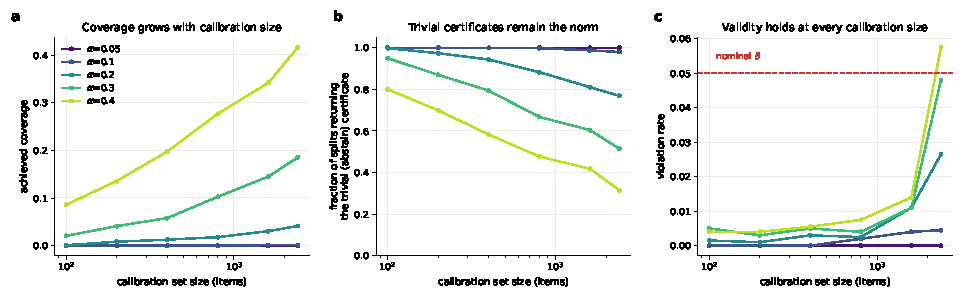
\includegraphics[width=0.98\textwidth]{figs/fig6_calibration_size.pdf}
\caption{\textbf{More practice questions help slowly.} \textbf{(a)} Mean coverage against the number of practice questions, one line per budget $\alpha$. \textbf{(b)} Share of silent deployments. \textbf{(c)} Share of deployments that broke the promise. The dashed line is the 5\% limit. At 2{,}400 questions the 40\% budget reaches 5.8\%.}
\label{fig:calsize}
\end{figure}

\section{4-bit models}

Qwen2.5 1.5B and 3B were run in both 16-bit and 4-bit form on the same questions. Their answers agree on 84.9\% of questions on average, from 77.9\% on MedMCQA to 93.6\% on PubMedQA. The mean change in area under the risk--coverage curve is 0.031. That is small next to the 0.27 spread across configurations (Figure~\ref{fig:models}a). Figure~\ref{fig:quant} breaks this down by benchmark.

\begin{figure}[H]
\centering
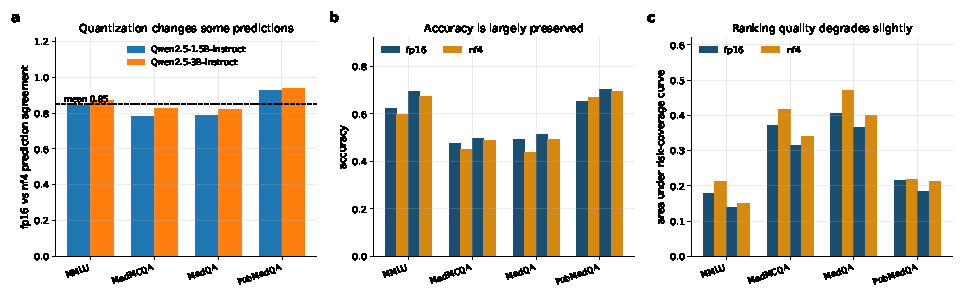
\includegraphics[width=0.98\textwidth]{figs/fig7_quantization.pdf}
\caption{\textbf{4-bit models cost a little.} \textbf{(a)} Agreement between 16-bit and 4-bit answers on the same questions, for the two configurations run both ways, with the overall mean. \textbf{(b)} Accuracy in each form by benchmark. \textbf{(c)} Area under the risk--coverage curve in each form by benchmark (lower is better). The 4-bit bars sit slightly higher, a small and even cost.}
\label{fig:quant}
\end{figure}

\section{Scope and limits}

\begin{itemize}[leftmargin=1.4em]
    \item \textbf{Small models by design.} We study models that fit on one 16\,GB graphics card, because hospitals can run them on their own hardware. The 7B models run in 4-bit form. Larger models are more accurate and may speak more often. By Proposition~\ref{prop:silence}, that would shrink the gap. We do not test them.
    \item \textbf{Multiple choice.} The model picks from listed options. Our results apply to that format, not to free-text medical advice.
    \item \textbf{The model's own confidence.} Confidence comes from the model's answer probabilities. Its overconfidence and its sensitivity to option order are part of what we measure.
    \item \textbf{140 new questions.} We judge each deployment on 140 new questions, while the theory concerns all future questions. This adds noise to the measured failure rates. The noise is symmetric. So it cannot explain why new questions went worse in 68\% to 98\% of speaking deployments instead of 50\%.
    \item \textbf{Estimated weights.} The reweighting fix uses weights estimated by a classifier. Because it never spoke, we cannot tell weight errors apart from the caution of its bound.
    \item \textbf{Contamination.} Benchmark questions may appear in a model's training data. That would raise coverage on those benchmarks. We cannot detect it from the answers alone.
\end{itemize}

\end{document}
